\scanpage{50}
biextension \deleted{\unsure{de}} de $P,Q$ par $G$, et où $(E',\varphi)$ est le couple d'une biext. $E'$ de $P',Q$ par $G$ et d'un hom
\diagram{\begin{tikzcd}[ampersand replacement=\&]\varphi:T_\Pi(P)\times T_\Pi(Q)\arrow[r]\&T_\Pi(G)\end{tikzcd}}
\uline{qui étend l'hom}
\diagram{\begin{tikzcd}[ampersand replacement=\&]\deleted{\unsure{\varphi}}\ \varphi_{\Pi,E'}:T_\Pi(P')\times T_\Pi(Q)\arrow[r,no head]\&T_\Pi(G)\end{tikzcd}}

\margin{\fbox{\begin{minipage}{.65\linewidth}
$\unsure{2}$\quad\uline{NB} On considère les $T_\Pi(P)$ comme syst. projectifs \deleted{par suite} \deleted{\uline{\unsure{stricts}}}, \inserted{\unsure{elle est vraie}} cette description \unsure{ne marche que} \deleted{\unsure{en} \unsure{termes} de syst. projectifs (\unsure{sans passage à la limite})} si $\forall p\in\Pi$ on a $pP'=P'$, $\unsure{pP''=pP''|pP''=P''}$ donc $\unsure{pP=pP|pP=P}$. Sinon, il faut garder le syst. des ${}_nP\times{}_nQ\mathbin{-}{}_nG$ \deleted{\unsure{prolongeant} ${}_nP'\times{}_nQ\mathbin{-}{}_nG$} avec la compatibilité \unsure{pour} \deleted{\unsure{un et}} \uline{\unsure{et}} la compatibilité \unsure{des restrictions} aux $\deleted{\unsure{\times}}{}_nP'\times{}_nQ\ \ldots$
\end{minipage}}}

\uline{Corollaire 1} Soient deux suites exactes
\diagram{\begin{tikzcd}[ampersand replacement=\&, column sep=small]
0\arrow[r,no head]\&P'\arrow[r,no head]\&P\arrow[r,no head]\&P''\arrow[r,no head]\&0\\
0\arrow[r,no head]\&Q'\arrow[r,no head]\&Q\arrow[r]\&Q''\arrow[r]\&0
\end{tikzcd}}
et supposons que, pour un $\Pi$ de nbs premiers, on ait :
\[
\text{a)}\quad p\in\Pi\Longrightarrow\uline{pP=P},\quad\uline{pQ'=Q'}\quad
\deleted{\unsure{et}\ pQ''=Q''\ \unsure{ou}\ pP''=P''}
\]
\inserted{(ou le symétrique)}
\margin{\deleted{(donc $pP=P$, $pQ=Q$)}}
\[
\text{b)}\quad\text{les}\quad\varinjlim_{n\to\Pi}{}_nP\longrightarrow P''\quad\text{et}\quad
\varinjlim_{n\to\Pi}{}_nQ\mathbin{-}Q''\quad\text{épim.}
\]
\figure{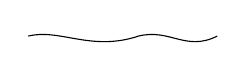
\begin{tikzpicture}\draw (0,.1)..controls (.4,.2) and (.8,-.1)..(1.4,.1)..controls (1.8,.2) and (2,-.1)..(2.4,.1);\end{tikzpicture}}
\margin{\fbox{\begin{minipage}{.65\linewidth}
\unsure{Ne vaut que}, celle en modules tel quel que si on suppose que $P',Q;P'',Q'$ sont $\Pi$ divisibles dans a), en plus de b). Sinon, garder les ${}_nP\times{}_nQ\longrightarrow{}_nG\ \ldots$
\end{minipage}}}

Alors le foncteur
\diagram{\begin{tikzcd}[ampersand replacement=\&]E\arrow[r,mapsto]\&(E',\varphi)\end{tikzcd}}
\unsure{associant à} les biext. de $P,Q$ par $G$ \unsure{la restriction} $E':P',Q'$ et la forme $\varphi_{E,\Pi}$
\diagram{\begin{tikzcd}[ampersand replacement=\&]\varphi:T_\Pi(P)\times T_\Pi(Q)\arrow[r,no head]\&T_\Pi(G)\end{tikzcd}}
prolongeant
\diagram{\begin{tikzcd}[ampersand replacement=\&]\varphi_{E',\Pi}:T_\Pi(P')\times T_\Pi(Q')\arrow[r,no head]\&T_\Pi(G)\end{tikzcd}}
est une équivalence de catégories.

\uline{Dém.} \inserted{Supposons p.ex.} On applique d'abord le \deleted{\unsure{proposition}} corollaire 1 à
\diagram{\begin{tikzcd}[ampersand replacement=\&, column sep=small]0\arrow[r,no head]\&P'\arrow[r]\&P\arrow[r,no head]\&P''\arrow[r,no head]\&0\end{tikzcd}}
et $Q'$, en utilisant $pQ'=Q'$, $\varinjlim{}_nP\longrightarrow P''$ épim.

Cela donne une description des biextensions de $P,Q'$. On applique ensuite le sym. du cor. 1 à $P$ et
\diagram{\begin{tikzcd}[ampersand replacement=\&, column sep=small]0\arrow[r,no head]\&Q'\arrow[r]\&Q\arrow[r]\&Q''\arrow[r]\&0\end{tikzcd}}
en utilisant $pP=P$ \deleted{$\unsure{pP''=P''}$} et $\varinjlim_{n\to\Pi}{}_nQ\mathbin{-}Q''$ épim.
\margin{49}
